% Asset ID: AS1GraphsTransformationsTikZ-006
% Source: CCEA AS1-AF-LO016 + DrFrost coordinate-effects transcript
% Purpose: Point transformation table for common graph transformations
\documentclass[tikz,border=8pt]{standalone}
\usepackage{amsmath}
\usepackage{array}
\begin{document}
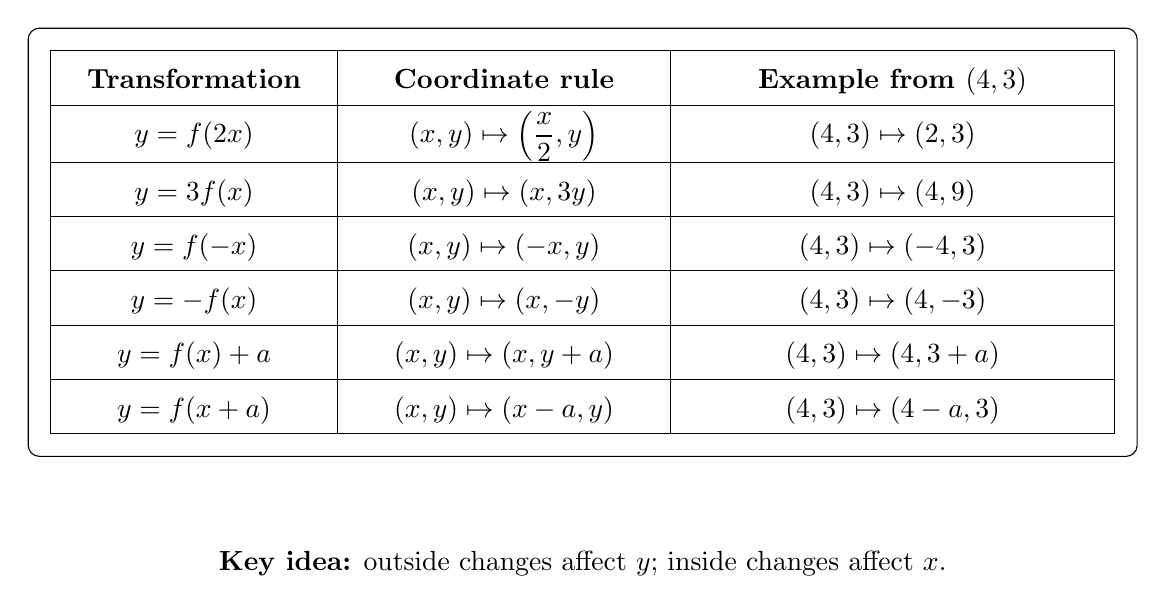
\begin{tikzpicture}
\node[draw,rounded corners,fill=white,inner sep=8pt]{\renewcommand{\arraystretch}{1.6}\begin{tabular}{|>{\centering\arraybackslash}m{3.2cm}|>{\centering\arraybackslash}m{3.8cm}|>{\centering\arraybackslash}m{5.2cm}|}\hline\textbf{Transformation}&\textbf{Coordinate rule}&\textbf{Example from $(4,3)$}\\\hline$y=f(2x)$&$(x,y)\mapsto\left(\dfrac{x}{2},y\right)$&$(4,3)\mapsto(2,3)$\\\hline$y=3f(x)$&$(x,y)\mapsto(x,3y)$&$(4,3)\mapsto(4,9)$\\\hline$y=f(-x)$&$(x,y)\mapsto(-x,y)$&$(4,3)\mapsto(-4,3)$\\\hline$y=-f(x)$&$(x,y)\mapsto(x,-y)$&$(4,3)\mapsto(4,-3)$\\\hline$y=f(x)+a$&$(x,y)\mapsto(x,y+a)$&$(4,3)\mapsto(4,3+a)$\\\hline$y=f(x+a)$&$(x,y)\mapsto(x-a,y)$&$(4,3)\mapsto(4-a,3)$\\\hline\end{tabular}};
\node[anchor=north,align=center] at (0,-3.8){\textbf{Key idea:} outside changes affect $y$; inside changes affect $x$.};
\end{tikzpicture}
\end{document}
